%%%%%%%%%%%%%%%%%%%%%%%%%%%%%%%%%%%%%%%%%%%%%%%%%%%%%%%%%%%%%%%%%%%%%%%%%%%%%%%%
%2345678901234567890123456789012345678901234567890123456789012345678901234567890
%        1         2         3         4         5         6         7         8
%% memo.tex
%% V1.1
%% 
%% 
%% based on a template created by Rob Oakes
%% customized for IST Courses by Rui Santos Cruz
%%%%%%%%%%%%%%%%%%%%%%%%%%%%%%%%%%%%%%%%%%%%%%%%%%%%%%%%%%%%%%%%%%%%%%%%%%%%%%%%
%-----------------------------------------------------------------------
%Aterado por JPAlves 2018 
%-----------------------------------------------------------------------
\documentclass[a4paper,10pt]{texRel}
\usepackage[english,main=portuguese]{babel} % Defines Main language
\usepackage[utf8]{inputenc}
\usepackage[T1]{fontenc}
\usepackage{iflang}
\usepackage{ifthen}
\usepackage{parskip}
\usepackage{matlab}
\usepackage{CPP}
\usepackage{python}
\usepackage{courier}
\usepackage{setspace}
\usepackage{multirow}
\usepackage{color}
\usepackage{array}
\usepackage{supertabular}
\usepackage{hhline}
\usepackage[siunitx]{circuitikz}
\pagestyle{plain}

\usepackage{titlesec}
\usepackage{graphicx,subfigure,ulem,float}
\usepackage{amsmath,amssymb,amsfonts}

\setlength{\parindent}{11pt}
\DeclareUnicodeCharacter{00B1}{\pm}
\logo{
\includegraphics[width=0.2\textwidth]{imagens/logo/image001.jpg}} % Logo
\titleformat{\chapter}[display]
    {\normalfont\huge\bfseries}{\chaptertitlename\ \thechapter}{20pt}{\Huge}
\titlespacing*{\chapter}{0pt}{0pt}{40pt}
\providecommand{\keywords}[1]{\noindent \textbf{\textit{Palavras chave:}} #1}

\makeatother
%%%%%%%%%%%%%%%%%%%%%%%%%%%%%%%%%%%%%%%%%%%%%%%%%%%%%%%%%%%%%%%%%%%%%%%%%%%%%%%%
%	MEMO INFORMATION --> Write your info in the following tags.
%%%%%%%%%%%%%%%%%%%%%%%%%%%%%%%%%%%%%%%%%%%%%%%%%%%%%%%%%%%%%%%%%%%%%%%%%%%%%%%%
\memofrom{João Pedro Antunes Pereira Rodrigues Alves} % Sender(s) Name
%\memoid{} %ID do aluno
%\memocourse{} %Disciplina

%----------------------------------------------------------------------------------
\memoorient{António Valente, Nuno Miguel Fonseca Ferreira}
%----------------------------------------------------------------------------------

\memosubject{ Sistemas inteligentes para a condução autónoma, demonstrador aplicado à robótica móvel} % Assunto 
\memodate{\today} % Date, -> set to \today for automatically print todays date
%%%%%%%%%%%%%%%%%%%%%%%%%%%%%%%%%%%%%%%%%%%%%%%%%%%%%%%%%%%%%%%%%%%%%%%%%%%%%%%%
\usepackage[square,sort,comma,numbers]{natbib}
\usepackage{hyperref}
%\renewcommand{contentsname}{índice}
\bibliographystyle{unsrtnat}
\setcounter{tocdepth}{1}
\begin{document}
\maketitle

\tableofcontents
\begin{abstract}
Temos testemunhado nos últimos anos um progresso vertiginoso em relação à inteligência artificial relacionada com os campos tais como visão computacional, aprendizagem (aprendizado??) de máquina e veículos autónomos. ... Pretende-se construir uma Plataforma ...
%%%%%%%%%%%%%%%%%%%%%%%%%%%%%%%%%%%%%%%%%%%%%%%%%%%%%%%%%%%%%%%%%%%%%%%%%%%%%%%%%%%
falta texto
%%%%%%%%%%%%%%%%%%%%%%%%%%%%%%%%%%%%%%%%%%%%%%%%%%%%%%%%%%%%%%%%%%%%%%%%%%%%%%%%%%%


---- é uma plataforma flexível e de baixas expensas para educação autónoma e investigação é composta por pequenos veículos autónomos e cidades construidos com componentes de prateleira, cidades as quais são constituídas por estradas com sinalização rodoviária, semáforos, obstáculos e cidadãos com necessidade de transportes. 
     
\noindent A plataforma oferecerá um leque variado de funcionalidades a baixo custo os robots percecionam o mundo em redor através de uma webcam monocular e fazem parte do processamento numa raspberry pi 3, contudo são capaz de seguir uma linha enquanto evitam obstáculos sejam pedestres ou outros robots ...  [duck1]


Duckietown is an open, inexpensive and flexible
platform for autonomy education and research. The platform
comprises small autonomous vehicles (“Duckiebots”) built from
off-the-shelf components, and cities (“Duckietowns”) complete
with roads, signage, traffic lights, obstacles, and citizens (duck-
ies) in need of transportation. 


The Duckietown platform offers
a wide range of functionalities at a low cost. Duckiebots sense
the world with only one monocular camera and perform all
processing onboard with a Raspberry Pi 2, yet are able to:
follow lanes while avoiding obstacles, pedestrians (duckies) and
other Duckiebots, 


localize within a global map, navigate a
city, and coordinate with other Duckiebots to avoid collisions.
Duckietown is a useful tool since educators and researchers
can save money and time by not having to develop all of
the necessary supporting infrastructure and capabilities. All
materials are available as open source, and the hope is that
others in the community will adopt the platform for education
and research.

Self-driving vehicles are poised to become one of the most
pervasive and impactful applications of autonomy. However,
difficult challenges still remain before their widespread deploy-
ment, many of which concern the system as a whole, rather
than single components in isolation. Examples include the co-
design of hardware components and algorithms, the coupled
interactions between perception and control, the optimal
allocation of finite computational resources to concurrent
processes, and safe multi-agent behaviors.
\begin{tikzpicture}[scale=2]
  \draw[color=black, thick]
    (0,0) to [short,o-] (6,0){} % Baseline for connection to ground
    % Input and ground
    (0,1) node[]{\large{\textbf{INPUT}}}
    % Connection of passive components
    (5,0) node[ground]{} node[circ](4.5,0){}
    (0,2) to [pC, l=$C_1$, o-] (0.5,2)
    to [R,l=$R_1$,](1.5,2)
    to node[short]{}(2.6,2)
    (1.5,2) to [C, l=$C_2$, *-] (1.5,3) -| (5,3)
    (2.2,2) to [R, l=$R_2$, *-*] (2.2,3)
    (2.2,3) to [pC, l=$C_3$, *-] (2.2,5) -| (3,5)
    % Transistor Bipolar Q1
    (3,0) to [R,l=$R_5$,-*] (3,1.5)
    to [Tnpn,n=npn1] (3,2.5)
    (npn1.E) node[right=3mm, above=5mm]{$Q_1$} % Labelling the NPN transistor
    (4,0) to [pC, l_=$C_4$, *-] (4, 1.5)--(3,1.5)
    (2.2,0) to [vR, l=$R_3$, *-*] (2.2,2)
    (3,2.5) to node[short]{}(3,3)
    (3,5) to [pR, n=pot1, l_=$R_4$, *-] (3,3)
    (3,5) to [R, l=$R_6$, *-] (5,5)
    to [short,*-o](5,5.5) node[right]{$V_S=40 V$}
    % Mosfet Transistors
    (5,3) to [Tnigfetd,n=mos1] (5,5)
    (mos1.B) node[anchor=west]{$Q_2$} % Labelling MOSFET Q2 Transistor
    (pot1.wiper)  to [R, l=$R_7$] (4.5,4) -| (mos1.G)
    (5,1.5) to [Tpigfetd,n=mos2] (5,2.5)
    (5,0) to (mos2.S)
    (3,2.5) to [R, l=$R_8$, *-] (4.5,2.5)
    -| (mos2.G)
    (mos2.B) node[anchor=west]{$Q_3$} % Labelling MOSFET Q3 Transistor
    % Output
    (6,3) to [pC, l=$C_5$,-*](5,3)
    (6,3) to [short,-o] (6,2){}
    (mos1.S)--(mos2.D)
    (6,0) to [short,-o] (6,1){} node[above=7mm]{\large{\textbf{SPEAKER}}}
    ;
\end{tikzpicture}
\keywords{Condução autónoma, Inteligência artificial, Plataforma, four}
\end{abstract}

\chapter{Motivação}

\section{Introdução}

A condução é uma actividade cada vez mais presente no nosso dia-a-dia e sujeita a cada vez mais estudos e avanços tecnológicos. Trata-se de uma actividade extremamente complexa, do ponto de vista cognitivo, que requer atenção, alerta, concentração, coordenação olho-mão-pé e a capacidade de processar informação visual, cinestética e auditória em simultâneo. Segundo os dados da OMS, mais de 1.2 milhões de pessoas morrem nas estradas, todos os anos, tornando esta uma das principais causas de morte na Europa. Para além de ser um problema de saúde pública é ainda um problema ao nível económico, acarretando um custo de cerca de 3\% do produto interno bruto \cite{Geneva}. Apesar de, nos últimos anos (2010-2016) Portugal ter verificado uma redução de cerca de 40\% relativamente aos mortos nas estradas, a tendência parece estar a inverter-se uma vez que só no primeiro trimestre de 2018 já se verificou um aumento no número de acidentes rodoviários e mortos nas estradas portuguesas, em comparação com o ano de 2017 \cite{PT1}. 

Apesar destes valores, a maior parte dos acidentes rodoviários são previsíveis e evitáveis, pelo que vários países se têm empenhado na criação de medidas e estratégias de forma a diminuir o número de acidentes rodoviários e a aumentar a segurança nas estradas. Portugal é um dos países que procura, de forma ativa, combater de forma sistemática a insegurança rodoviária através dos seguintes planos: Plano Integrado de Segurança Rodoviária (PISER, 1998-2000), Plano Nacional de Prevenção Rodoviária (PNSR, 2003-2010) e Estratégia Nacional de Segurança Rodoviária (ENSR, 2008-2015) \cite{DR}.
Verificou-se, no entanto, que mesmo após execução da Estratégia Nacional de Segurança Rodoviária (2008-2015), alguns dos principais problemas relacionados com esta temática ficaram por resolver como é o caso de questões como: "O estabelecimento de questões de políticas integradas de comunicação que tenham impacto eficaz e eficiente nas atitudes e comportamentos de todos os utilizadores do Sistema de Transporte Rodoviário; 
O melhor conhecimento da sinistralidade e das suas causas, através do cruzamento dos dados estatísticos e participações de acidentes, recolhidos pelas forças de segurança e pelas unidades de saúde; 
A identificação e aplicação de um processo que melhore a avaliação do risco da infraestrutura rodoviária; e ainda, a definição e aplicação de uma política nacional de fiscalização baseada nas melhores práticas internacionais." \cite{DR}.

É neste âmbito que surge o programa PENSE2020, cuja elaboração contou com a participação de diversos serviços da administração publica, central e local, bem como de organizações não governamentais da área da segurança rodoviária e está assente na ideia de que as políticas públicas de segurança rodoviária necessitam de estar suportadas em estratégias eficazes e eficientes que envolvam e motivem a sociedade, tendo o objetivo de garantir maior segurança para os utilizadores, tornar as infraestruturas e os veículos mais seguros e ainda melhorar a assistência e apoio às vítimas. Este programa conta com cinco grandes objetivos estratégicos focados nestas preocupações e na sua resolução: 
\begin{description}
	\item [(1)] Melhorar a Gestão da Segurança Rodoviária; 
	\item [(2)] Fazer com que os Utilizadores se sintam mais seguros; 
	\item [(3)] Tornar mais seguras as infraestruturas; 
	\item [(4)] Veículos mais seguros e; 
	\item [(5)] Melhorar a Assistência e apoio ás vítimas. 
\end{description}

Desdobrando o primeiro objetivo estratégico, podemos encontrar três objetivos operacionais dois dos quais se relacionam com a proposta de investigação que apresentamos neste documento: 
%%%%%%%%%%%%%%%%%%%%%%%%%%%%%%%%%%%%%%%%%%%%%%%%%%%%%%%%%%%%%%
\begin{description}
\item[(1)] Melhorar o Sistema de recolha, tratamento e disponibilização de informação sobre segurança rodoviária; 
\item[(2)] Desenvolver um demonstrador robótico para validação das diversas estratégias de apoio à condução autonoma nas cidades.
\end{description} 
%%%%%%%%%%%%%%%%%%%%%%%%%%%%%%%%%%%%%%%%%%%%%%%%%%%%%%%%%%%%
Este programa apresenta, ainda, a vontade de que o seu resultado final seja o de que "ninguém deve morrer ou ficar permanentemente incapacitado na sequência de um acidente rodoviário em Portugal"  \cite{DR}.
É fundamental que as estratégias e políticas adotadas se foquem também no fator humano, que está presente em quase todos os acidentes rodoviários, sendo que os principais riscos são: 
\begin{itemize}
\item   excesso de velocidade;
\item   uso de capacete para o caso dos motociclistas;
\item 	uso do cinto de segurança;
\item	condução sob o efeito de álcool; 
\item 	condução sob o efeito se substâncias psicotrópicas; 
\item	proteção adequada das crianças;
\item   condução distraída e desatenta associada a, por exemplo, condução ao telemóvel. 
\end{itemize}

%-----------------------------------------------------------------------------------------------\\


\chapter{A evolução da condução autónoma}


\section{Introdução}

Quando se fala de condução autónoma, fala-se da técnica que tem como objetivo a automatização, total ou parcial, de várias tarefas relacionada com a condução [xx1] por forma a proporcionar ao utilizador uma experiência do tipo taxi, no entanto, haver necessidade para a existência de um condutor.
Porém, a condução autónoma representa um desenvolvimento que não se fica pela componente tecnológica. De facto esta apresenta benefícios a nível social e económico, uma vez que a sua área de interesse inclui sistemas de segurança ativa e passiva, sistemas auxiliares à condução (no casos de condições de condução específicas ou de utilizadores que apresentem algum tipo de deficiência ou incapacidade para conduzir) e sistemas que possibilitem a otimização da utilização das infraestruturas e recursos energéticos disponíveis.
Ao falar-se de veículos autónomos, está então a falar-se de uma família de tecnologias altamente automatizadas e concebidas para minimizar (e em alguns casos até evitar) acidentes e lesões, permitir uma melhor exploração da rede de estradas, reduzir o consumo energético, permitir uma maior e melhor mobilidade, ou mesmo reduzir o custo associado ao transporte de bens e mercadorias.
Pensa-se que a implementação deste tipo de sistemas, aliada à utilização de formas de propulsão amigas do ambiente, seja o maior avanço na tecnologia automóvel até ao ano 2020.


Em 1964 a 1971 Stanford Cart foi pioneiro por apresentar técnicas para navegar através de um ambiente desconhecido através de sistemas com inteligência artificial e visão.
\begin{figure}[H]
\centering
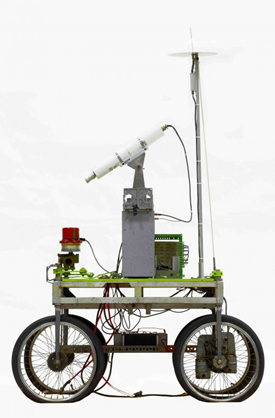
\includegraphics[width=55mm,scale=0.5]{imagens/cap2/Stanford_AIL_1964.png}
\caption{O primeiro robô autónomo.}
\label{fig1}
\end{figure}

O primeiro veículo autónomo foi construído em 1977, no Laboratório de Engenharia Mecânica da Universidade de Tsukuba, no Japão. Tratava-se de um carro dotado com um sistema de visão computacional baseada em câmaras de televisão e uma unidade de processamento. Este sistema de visão permitia a deteção de obstáculos e seguir as linhas brancas marcadas nas estradas. Este veículo conseguia atingir velocidades de 30 Km/h \cite{Robocorp}. 

Para a época, este veículo autónomo constituiu um grande desafio, uma vez que os computadores ainda tinham uma capacidade de processamento muito limitada.

Em 1980, uma carrinha Mercedes-Benz, desenhada por Ernst Dickmanns e pela sua equipa na Universidade de Bundeswehr em Munique, atingiu, usando visão, os 100 km/h numa rua sem trânsito. Após esta experiência, a Comissão Europeia começou a patrocinar o projeto EUREKA Prometheus (1987-1995), projeto esse que foi o maior projeto de R\&D feito na área da condução autónoma, tendo recebido mais de mil milhões de dólares por parte a Comissão Europeia e que definiu o estado de arte em termos de veículos autónomos.

Ainda em 1980, o Autonomous Land Vehicle (ALV) patrocinado pela DARPA conseguiu, pela primeira vez, controlar um veículo sem intervenção humana, a uma velocidade de 30 km/h, usando radares laser, visão computorizada e um mecanismo robótico de controlo.

Em 1994, dois veículos robóticos, VaMP e Vita-2, conduziram mais de mil quilómetros numa autoestrada Parisiense de três vias de forma semiautónoma, em conduções típicas de trânsito intenso, atingindo a velocidade máxima de 130 km/h. Estes veículos demonstraram, ainda, a condução em faixas de rodagem desimpedidas, condução integrando uma coluna de veículos e mudanças de faixa, realizando de forma autónoma a ultrapassagem de outros veículos.



\begin{figure}[H]
\centering
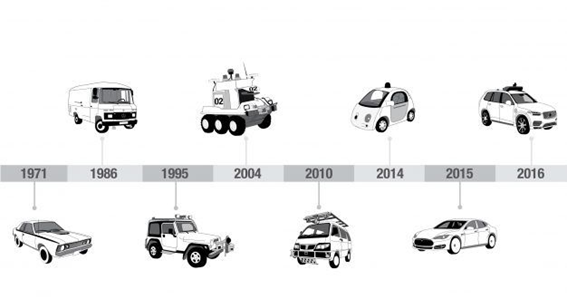
\includegraphics{imagens/cap2/time-line.png}
\caption{A evolução dos carros autónomos.}
\label{fig2}
\end{figure}


Em 1995, um Mercedes-Benz Classe S modificado por Dickmanns, realizou uma viajem de ida e volta entre Munique (Bavária) e Copenhaga (Dinamarca), num total de 1600 quilómetros, usando visão sacádica computadorizada (uma técnica que simula o comportamento do olho humano ao procurar por pontos de interesse numa imagem e recolhendo informação mais detalhada acerca desses pontos em particular, por forma a construir uma representação da imagem observada e ao mesmo tempo rentabilizar os recursos disponíveis) e transputers, de maneira a obter um controlo em tempo real. Durante este teste, o robô atingiu velocidades impressionantes de mais de 175 km/h na autoestrada Alemã, conduziu em condições normais de tráfego (executando manobras para ultrapassar outros veículos) e conseguiu conduzir 158 quilómetros sem intervenção humana, mesmo tratando-se de um sistema concebido para investigação e sem qualquer tipo de ênfase na fiabilidade em grandes deslocações.

Ainda em 1995, no âmbito do projeto Navlab da Universidade Carnegie Mellon (Pittsburgo, Pensilvânia, EUA), foram conseguidos 98,2\% de condução autónoma ao longo de um percurso com 5000 quilómetros (3000 milhas terrestres), numa viajem intitulada No hands across América. 
O veículo usado para realizar este percurso era, no entanto, apenas semiautónomo, uma vez que foram usadas redes neuronais para controlar automaticamente a direcao e a potência, mas os travões eram controlados por humanos.

Entre 1996 e 2001, o governo Italiano patrocinou o projeto ARGO[2], que decorreu na Universidade de Parma e foi coordenado pelo Professor Alberto Broggi. No âmbito deste projeto, procedeu-se à modificação de uma Lancia Thema para que este conduzisse autonomamente por seguimento das guias delimitadoras de faixa de rodagem existentes numa autoestrada típica, monitorizando o ambiente à sua volta por forma a localizar obstáculos no seu caminho e efetuando mudanças de faixas de rodagem. 

O projeto culminou com uma viagem batizada de MilleMiglia in Automático (em português, Mil Milhas em modo Automático) ao longo de 2000 quilómetros, durante seis dias, nas autoestradas do norte de Itália. Esta viajem caracterizou-se pela obtenção de uma velocidade média de 90 km/h, por 94\% da sua duração ter sido feita em modo automático e por se terem percorrido distâncias até 54 quilómetros sem intervenção humana. Em termos de tecnologia, para a condução foram apenas usadas duas câmaras de vídeo de baixo custo, a preto e branco, e algoritmos de visão estereoscópica (uma técnica que simula o comportamento do olho humano e usa a paralaxe para, através da fusão de duas imagens bidimensionais, conseguir uma noção de profundidade e a avaliação da distancia, posição e tamanho de objetos [3]) para que o veículo conseguisse compreender o ambiente em que se encontrava, muito diferente das abordagens de outras equipas de investigação.

Em 2001, um projeto do exército dos estados Unidos, denominado de Demo III, demonstrou a capacidade de veículos terrestres autónomos percorrerem distâncias em terrenos irregulares, evitando obstáculos tais como pedras e árvores. O sistema de controlo utilizado foi um sistema hierárquico, designado de Real-Time Control System e fornecido por James Albus da NIST. Foi ainda demonstrado que era possível não só controlar veículos individuais, mas também coordenar um conjunto de veículos por forma a atingir determinado objetivo.

Também em 2001, tem a sua primeira edição o maior encontro na área da robótica em Portugal, o Festival Nacional de Robótica. 

\begin{figure}[H]
\centering
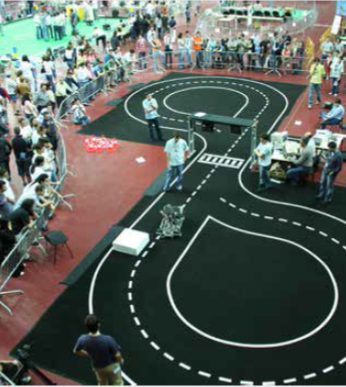
\includegraphics{imagens/cap2/FNR.png}
\caption{O Festival Nacional de Robótica em Portugal.}
\label{fign}
\end{figure}

Este evento, atualmente uma iniciativa da Sociedade Portuguesa de Robótica, tem como objetivo contribuir para o desenvolvimento da investigação em robótica e automação e promover a ciência e a tecnologia junto dos jovens em vários níveis de ensino, bem como do público em geral, através de competições entre robôs. O Festival decorre todos os anos numa cidade distinta e inclui um encontro científico, onde investigadores nacionais e estrangeiros, da área da robótica, se reúnem para apresentar os mais recentes resultados da sua atividade. Este evento tem tido desde o seu início um enorme crescimento, quer em termos de participantes, quer em termos de adesão do público [4]. 

Foi neste contexto que surgiu a prova de Condução Autónoma, a grande motivação deste trabalho, com o objectivo de fomentar a investigação e consequente desenvolvimento de técnicas que pudessem ser utilizadas na construção de veículos autónomos.

Em 2004, teve lugar a primeira edição de uma das maiores competições a nível mundial no que toca a condução autónoma, o DARPA Grand Challenge. 

Esta competição é patrocinada pela DARPA, a mais importante organização em termos de investigação do Ministério da Defesa Dos Estados Unidos, e consiste na competição entre equipas originárias de vários países, desde que um dos elementos da equipa seja um cidadão Americano, em corridas de veículos autónomos. Para promover ainda mais a competição e fomentar o interesse e empenho na investigação nesta área da robótica, o Congresso dos Estados Unidos, autorizou a DARPA a atribuir um prémio de um milhão de dólares ao vencedor da competição. Através deste incentivo, o Ministério da Defesa dos Estados Unidos pretendia conseguir acelerar o processo da criação de tecnologia que permitisse que, em 2015, pelo menos um terço de todos os veículos terrestres do exército fossem autónomos. 

Além do claro objectivo em termos militares (ao eliminar a componente humana na condução de veículos de combate, poderão salvar-se vidas nos campos de batalha), esta competição tem também objectivos em termos comerciais. Como consequência da investigação feita no âmbito desta competição, poderá ser possível, ao premir um botão, ser conduzido ao emprego, ou desenvolver sistemas que irão contribuir para aumentar o nível de segurança nos transportes, mesmo que eles não sejam totalmente autónomos.

Não se pode dizer que a primeira edição deste evento tenha sido um sucesso em termos competitivos, uma vez que das quinze equipas que se apresentaram em prova nenhuma das equipas chegou ao fim do percurso de 150 milhas (241 km) no deserto do Mojave (o veículo mais bem classificado percorreu uma distância de 11,78 km, cerca de 5\% da distância total), ficando o prémio de um milhão de dólares por reclamar. As suspeitas de que não iria haver grandes prestações começaram logo aquando dos testes preliminares, quando apenas setes das vinte e uma equipas qualificadas completaram a totalidade de um percurso com obstáculos. Foram treze as equipas que se apresentaram à partida para a corrida final, mas três horas após o início da competição, apenas quatro equipas continuavam em prova, não tardando muito até que todos os veículos tivessem desistido, sido desqualificados ou vítimas de falhas fatais. Travões presos, capotamento, eixos partidos e problemas com os dispositivos de localização por satélite, foram factores que levaram à exclusão de prova dos vários veículos.
Não obstante, a organização do evento estava bastante contente com os resultados obtidos, uma vez que, na sua opinião, tinha sido atingido o objectivo principal do evento, a promoção a nível mundial desta área da robótica, ao despertar o interesse de centenas de pessoas, desde curiosos, investigadores em universidades e empresas de carácter tecnológico.

Em Outubro de 2005 tem lugar a segunda edição do DARPA Grand Challenge. Nesta segunda edição, os vinte e três concorrentes, seleccionados de um grupo inicial de cento e noventa e cinco, reduzido para quarenta e três, após participação numa prova de qualificação com o nome de National Qualification Event (NQE), teriam de percorrer 212km num percurso off-road acidentado. 

Apesar de, em relação ao percurso da edição anterior, o percurso de 2005 não ter inclinações tão acentuadas (na edição anterior um dos veículos teve de desistir por não ter potência suficiente para ultrapassar um troço do percurso), os espaços para condução eram, em geral, mais estreitos e apresentavam curvas com um grau de dificuldade mais elevado. Apenas um dos veículos participantes na corrida final não ultrapassou o melhor registo da edição anterior, sendo que cinco veículos conseguiram completar a totalidade do percurso, quatro deles dentro do tempo limite (atingindo velocidades médias entre os 28.2 km/h e os 30.7 km/h).

O prémio para o vencedor da edição de 2005 do DARPA Grand Challenge foi de dois milhões de dólares, o dobro do anunciado para a edição anterior, e foi arrebatado por um VW Touareg da Universidade de Stanford, baptizado de Stanley, que percorreu a totalidade do percurso em seis horas e cinquenta e quatro minutos.

Em Maio de 2006, realiza-se a primeira edição do European Land-Robot Trial (ELROB), uma evento que, através de dois cenários, permite às equipas participantes a demonstração dos mais recentes avanços alcançados na construção de veículos terrestres autónomos, além de ser uma oportunidade de mostrar o estado de arte da robótica nos dias que correm.

Em Novembro de 2007 tem lugar a terceira edição do DARPA Grand Challenge. Esta edição, apelidada de Urban Challenge, teve lugar num recinto fechado (uma base aérea desmantelada) e consistiu num desafio diferente em relação às duas edições anteriores. Das oitenta e nove equipas que se candidataram a um lugar na corrida final, apenas trinta e cinco foram convidadas a participar no NQE. 

O National Qualifying Event para o Urban Challenge consistiu em oito dias de rigorosos testes, em três cenários diferentes, aos veículos candidatos. Numa primeira secção, era avaliada a capacidade dos veículos lidarem com situações de mudanças de direcção num circuito fechado de duas vias, com trânsito em ambos os sentidos. Numa segunda secção, eram avaliadas as capacidades de navegação, parqueamento e desvio de carros parados na via. Na terceira e última secção, os veículos tinham de lidar com cruzamentos, respeitando as regras de prioridade, e situações de estrada sem saída (para avaliar qual a capacidade dos robôs em recalcular um novo percurso para completar o objectivo pretendido). Após a fase de qualificação, foram seleccionadas, por motivos de segurança, apenas onze equipas. Destas onze equipas, seis chegaram ao fim e dentro do limite máximo de seis horas estabelecido para esta prova. 

As restantes foram desclassificadas por terem comportamentos de risco (situações de embate iminente com outros veículos ou com edifícios). O Urban Challenge constituiu, então, um enorme avanço na área da condução autónoma, na medida em que, pela primeira vez, interagiram num mesmo cenário veículos autónomos e veículos conduzidos pelo homem, sendo que todos eram obrigados a cumprir o código da estrada em vigor na Califórnia, estado onde decorreu a prova.

Em 2007 foram atribuídos prémios, num total de três milhões e quinhentos mil dólares, aos três primeiros classificados (dois milhões, um milhão e quinhentos mil dólares para o primeiro, segundo e terceiro classificados, respectivamente), tendo essas posições sido ocupadas pelo Chevy Tahoe da Universidade de Carnie Mellon (Pensilvânia) com o tempo de quatro horas, dez minutos e vinte segundos, pelo VW Passat SW da Universidade de Stanford (Califórnia) com quatro horas, vinte e nove minutos e vinte e oito segundos e pelo Ford Hybrid Escape do Instituto Politécnico e Universidade Estadual Virginia Tech (Virgínia) com o tempo de quatro horas, trinta e seis minutos e trinta e oito segundos.


De forma a incentivar a investigação nesta área (navegação autónoma), o governo Norte-americano em conjunto com a DARPA (Defense Advanced Research Projects Agency) criou um concurso internacional. Neste concurso de referência mundial, o objetivo dos veículos participantes é o de percorrerem um determinado trajeto num período de tempo limitado. Um dos mais conhecidos veículos participantes desta prova, designado “Stanley”, da equipa Stanford Racing Team, foi desenvolvido a partir de um Volkswagen Touareg R5 TDI, ilustrado na Figura \ref{fig:q} . 

\begin{figure}[H]
\centering
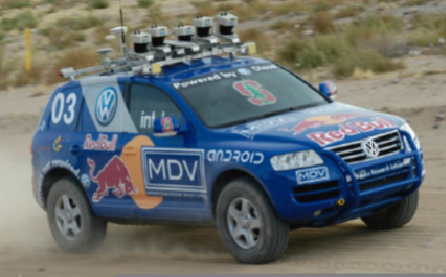
\includegraphics[width=85mm,scale=0.8]{imagens/cap2/stanley.png}
\caption{ O  Volkswagen Touareg R5 TDI da Stanford Racing Team.}
\label{fig_stanley1} \ref{fig:q}
\end{figure}

Em termos de sensores este veículo era constituído por duas unidades de navegação por GPS (Global Positioning System), cinco LADARs (Laser Detection and Ranging), dois radares, uma câmara de vídeo a cores, uma unidade de medição de inércia (IMU) constituída por três giroscópios e três acelerómetros. A informação gerada por este sistema sensorial era processada em seis computadores. Estes computadores eram também responsáveis pela navegação controlo do veículo. Este veículo venceu a prova DARPA Grand Challenge 2005, percorrendo 210,8 quilómetros no deserto de Mohave em 6 horas e 53 minutos [2].

Falar sobre a partilha de automóveis!
\begin{figure}[H]
\centering
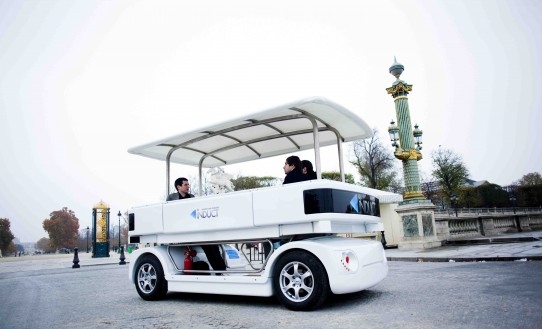
\includegraphics{future1.png}
\caption{Sistema de partilha de veiculos.}
\label{fig_futuro1}
\end{figure}

Falar sobre a utilização deste tipo de sistemas em ambientes estruturados
\begin{figure}[H]
\centering
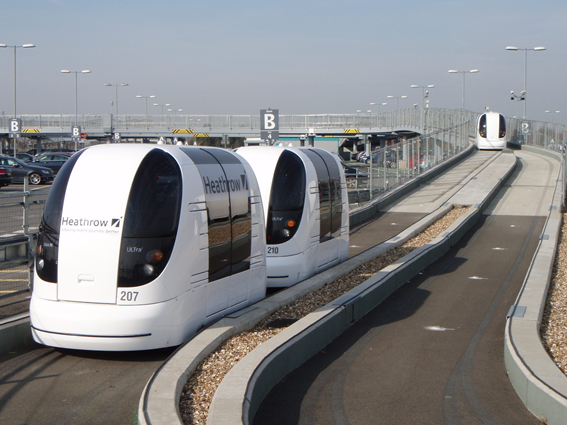
\includegraphics{future2.png}
\caption{Sistema de transportes inteligentes.}
\label{fig_futuro2}
\end{figure}

Falar sobre as vantagens dos diferentes niveis de automação e a qualidade de vida

A condução autónoma é suportada por veículos autónomos, considerados como veículos que se movem sem intervenção humana, interpretando o meio que os rodeia, e recorrendo a diversas tecnologias, como RADAR (Radio Detection And Ranging), LIDAR (Light Detection And Ranging), GPS, Odometria e Visão Computacional). Estes veículos são capazes de adaptar a sua condução em frações de segundos [23]. Os veículos autónomos encontram-se equipados com sistemas de condução autónoma e são descritos na literatura como “autónomos”, “sem motorista”, “robótico” ou “auto conduzido”. A SAE Internacional (antiga Sociedade de Engenheiros Automóveis) especifica 5 níveis de condução autónoma, e a Administração Nacional de Segurança de Transito nos EUA adaptou este sistema recentemente. Os 5 níveis de automação classificam-se da seguinte forma:
%%%%%%%%%%%%%%%%%%%%%%%%%%%%%%%%%%%%%%%%%%%%%%%%%%%%%%%%%%%%%%%%%%%%%%%%%%%%%%%%%%%%%%%%%%%%%%%%%%%
%Modificar

\begin{description}
\item[Nível 0 –] Sem automação: a condução do veículo depende da intervenção humana em tempo integral, para todos os aspetos de condução;  
\item[Nível 1 –] Assistência ao Motorista: o sistema, por vezes auxilia com tarefas específicas, como a escolha da direção ou aceleração e desaceleração, com o condutor humano realizando as restantes tarefas;
\item[Nível 2 –] Automação Parcial: o sistema executa tarefas, tais como escolha da direção juntamente com aceleração e desaceleração, sendo os humanos responsáveis pelas restantes tarefas;
\item[Nível 3 –] Automação Condicional: o sistema gere todas as tarefas e monitoriza o ambiente de condução, sendo que o ser humano só intervém quando o sistema requer assistência;
\item[Nível 4 –] Automação Elevada: o sistema conduz e monitoriza determinados ambientes e condições sem intervenção humana e é considerado totalmente autónomo em certos cenários, mesmo que o condutor humano não responda adequadamente a um pedido de intervenção;
\item[Nível 5 –] Automação Completa: o sistema faz tudo o que um motorista humano faz em todas as condições, combinando ou excedendo as capacidades de um humano em cada cenário de condução[24].
\end{description}
%%%%%%%%%%%%%%%%%%%%%%%%%%%%%%%%%%%%%%%%%%%%%%%%%%%%%%%%%%%%%%%%%%%%%%%%%%%%%%%%%%%%%%%%%%%%%%%%%%
 Recentemente, a indústria automóvel tem privilegiado o desenvolvimento de veículos mais seguros e confortáveis, o que estimula a procura de novos veículos inteligentes com controlo de condução autónoma.  
Um veículo autónomo é um veículo com condução autónoma que tem a capacidade de perceber o ambiente ao seu redor e realizar o controlo e planeamento do caminho sem a necessidade de intervenção humana.  
Em 2020, as multinacionais, General Motors, Volkwagem, Toyota e Google esperam vender veículos autónomos, e em 2035, prevê-se que 25% dos veículos que circularão nas estradas serão autónomos, beneficiando da cooperação de veículo-para-veículo.
Um veículo de condução autónoma está equipado com um módulo de comunicação apropriado, por exemplo, com comunicação DSRC e LTE, que suporta a troca de informação em tempo real entre veículos vizinhos, e entre veículos e estações de base. Além do módulo de comunicação, existem outros cinco módulos básicos que são necessários para apoiar a condução autónoma: a perceção, a localização, o planeamento, controlo e gestão do sistema [26].
A perceção é o processo que deteta o ambiente envolvente em torno do veículo autónomo, utilizando vários tipos de técnicas, tais como RADAR, LIDAR e computação visual que permitem a recolha de informação.  
O módulo de localização é implementado com o objetivo de encontrar a posição exata do veículo autónomo na estrada, utilizando o GPS (Sistema de Posicionamento Global), estimativas e mapas de estrada.
A função de planeamento determina o comportamento e movimento de um ADV (veículo de condução autónoma), com base nas informações obtidas através dos módulos de perceção e localização (Figura 9). Esta função planeia as rotas para cumprir a missão de viagem considerando tempo de viagem, distância e condição de tráfego.
O módulo de controlo é responsável pela execução dos comandos desejados pelo módulo de planeamento/gestão, controlando os atuadores, como por exemplo, direção, aceleração e travagem de um ADV.  
O módulo de gestão orienta comportamentos de condução, tais como mudança de faixa, comportamento a ser realizado numa interseção e comportamento de estacionamento, com base nas informações de trânsito e informação interna do veículo, a partir da função de perceção, enquanto segue a navegação a partir da função de planeamento. O módulo de gestão do sistema, tem também como função supervisionar o estado geral do sistema de um veículo autónomo, como por exemplo, a gestão de falhas, sistemas de login e interface homem-máquina (HMI) [27].

%%%%%%%%%%%%%%%%%%%%%%%%%%%%%%%%%%
\setlength{\tabcolsep}{0pt}
{\centering
Tabela 5: Tipo de mensagens de controlo autónomo (Adaptada de [26])
\par}


\begin{flushleft}
%\tablefirsthead{}
%\tablehead{}
\begin{center}
\begin{tabular}{m{4.794cm}|m{4.794cm}|m{4.795cm}}
\hline\multicolumn{1}{|m{4.794cm}|}{\centering \textbf{Tipo de Mensagens}} & \centering \textbf{Conteúdo das Mensagens} &\multicolumn{1}{m{4.795cm}|}{\centering\arraybslash \textbf{Exemplos}}\\\hline


\multicolumn{1}{|m{4.794cm}|}{\centering PSMs} &\begin{tabular}{m{4.795cm}}\begin{center} Posição \end{center} \\\hline \begin{center}\vspace{2mm} Direcção \end{center}\\\hline \begin{center}\vspace{2mm} Velocidade \end{center}\\\hline \begin{center}\vspace{5mm} Mau funcionamento\end{center} \end{tabular}&\multicolumn{1}{m{4.795cm}|}{
\vspace{1mm}
\begin{description}
\item Exemplo1. Quando ADVs circulam na estrada, precisam transmitir as PSMs em intervalos apropriados. 
\item Exemplo2. Quando qualquer ADV não se encontra em correto funcionamento, este precisa transmitir mensagens de mau funcionamento para ADVs próximos, a fim de estes manterem uma certa distância de segurança.
\end{description}


}\\\hline
\multicolumn{1}{|m{4.794cm}|}{\centering ATMs} &\begin{tabular}{m{4.795cm}}\begin{center}{ Mudar de faixa}\end{center} \\\hline \begin{center}\vspace{2mm}Ultrapassar \end{center} \\\hline \begin{center}\vspace{2mm} Travar \end {center}\\\hline \begin{center}\vspace{2mm}{Aviso de veículo de Emergência} \end{center}\end{tabular}&\multicolumn{1}{m{4.795cm}|}{
\vspace{1mm}
\begin{description}
\item Exemplo1. ADV 1 transmite ATMs para alertar os veículos vizinhos da sua intenção de ultrapassar, antes de ultrapassar. 

\item Exemplo 2. Quando um veículo de emergência entra num segmento rodoviário, é necessário transmitir ATMs para outros ADVs lhe forneçam prioridade
\end{description}

}\\\hline
%\tabletail{}
%\tablelasttail{}
\end{tabular}
\end{center}
\end{flushleft}

%%%%%%%%%%%%%%%%%%%%%%%%%%%%%%%%%%%

Apesar dos desenvolvimentos verificados, existem ainda vários desafios aos quais a condução autónoma deve dar resposta, tais como:

\begin{itemize}
\item	Ter conhecimento da posição exata do veículo e decidir como chegar ao destino;
\item	Detetar de forma eficiente o ambiente circundante para evitar a colisão do veículo;
\item	Detetar os sinais de trânsito, travessias, passadeiras, colisões etc [26].
\end{itemize}

Atualmente, para enfrentar estes desafios, além dos sensores utilizados no módulo de perceção, um novo “sensor” de longo alcance, a comunicação V2X, permite novos níveis de condução autónoma [28].
A comunicação V2X (Veículo-para-Tudo), também conhecida como Cooperative Connected Vehicles e Cooperative ITS, engloba os veículos que trocam dados entre si e com a infraestrutura, com o objetivo de melhorar a segurança rodoviária, aumentar a eficiência do tráfego, reduzir os impactos ambientais e fornecer serviços adicionais aos ocupantes do veículo.
As comunicações V2X são de quatro tipos: V2V (Vehicle-to-Vehicle), V2I (Vehicle-to-Infraes-truture), V2N (Vehicle-to-network) e V2P (Vehicle-to-pedestrian). A Figura 10 ilustra essas tipologias. Está implícito que estas comunicações são geralmente bidirecionais, isto é, por exemplo as comunicações V2I e V2N envolvem também o envio de mensagens da infraestrutura para os veículos.

As comunicações V2V e V2P baseiam-se essencialmente na capacidade de transmissão entre veículos ou entre veículos e utentes vulneráveis da estrada (por exemplo, pedestre, ciclista), com o objetivo de fornecer informações sobre a localização, velocidade e trajeto para evitar acidentes.  
A comunicação V2I ocorre entre um veículo e um RSU. Este tipo de comunicação pode incluir a comunicação entre veículos e dispositivos de controlo de tráfego, e nas proximidades de trabalhos rodoviários.
A comunicação V2N ocorre entre um veículo e um servidor de aplicação V2X, esta comunicação pode incluir a comunicação entre o veículo e o servidor via rede 4G / 5G, como para operações de tráfego.
As tecnologias utilizadas pela V2X incluem a WAN tradicional (Wireless Access Network) e as comunicações Wi-Fi, bem como o WAVE (Wireless Access in Vehicular Environments), baseado na DSRC para as camadas mais baixas e, nas comunicações moveis como é o exemplo do LTE.
A comunicação V2X permitir a partilha automática de informação em tempo real entre os utilizadores da estrada, promete melhorar significativamente a segurança rodoviária e minimizar os poluentes e combustível, bem como maximizar o uso eficiente das estradas e outras infraestruturas de transporte.
Por exemplo, os veículos e os seus ocupantes podem ter conhecimento das fases do sinal de trânsito, das zonas de trabalho rodoviário e dos perigos da estrada. Algumas dessas informações já estão disponíveis, como por intermédio de aplicações móveis. A comunicação V2X iria fornecer, no entanto, ainda mais informações, como diversas opções adicionais aos motoristas e veículos, que os sistemas de hoje não podem suportar. Outro exemplo, é permitir que municípios comuniquem aos veículos com as vagas de estacionamento disponíveis, por forma a reduzir o tráfego, evitando que os motoristas circulam sem parar no mesmo local a fim de obter um lugar de estacionamento, aumentando o congestionamento.
As comunicações V2X podem ser vistas como outro sensor no veículo. Enquanto outros sensores ativos como o RADAR, o LIDAR e o Computer Vision estão ativamente verificando o ambiente ao redor do veículo autónomo, o sensor sem fio V2X, com capacidade quando não existe linha de visão, está ativamente "ouvindo" e também "conversando" com outros carros para percecionar melhor o que está a acontecer em torno do veículo, recolhendo também informação sobre a intenção do condutor.
Outro benefício dos serviços V2X é que estes permitem a comunicação entre os ocupantes do veículo e o seu ambiente. Isto dá aos ocupantes acesso aos seus próprios dados e meios de comunicação e acesso à Internet no automóvel, o que permite uma vasta gama de novas aplicações e serviços [28].
Um carro robótico requer uma gama de tecnologias de sensores e comunicação V2X, sendo que todas estas tecnologias têm diferentes alcances de visão, e cada tecnologia tem um propósito dedicado que é comparável a um ou mais dos 5 sentidos humanos. O principal “sentido” de um carro robótico é o LIDAR, um processo baseado em laser que deteta objetos no ambiente próximo do carro, fornecendo informações de alta resolução sobre o ambiente em redor do carro. A importância deste sistema vem da sua precisão, possível até um intervalo de 100 metros, da sua capacidade de rotação de 360º e das mais de dois milhões de leituras por segundo. O segundo sentido de um carro robótico é o GPS, que permite a localização aproximada do carro, sendo que esta localização serve de base para sistemas de navegação. Embora seja uma tecnologia avançada, a precisão do GPS é insuficiente para a próxima geração de carros com condução autónoma, no melhor dos casos o GPS atinge uma precisão de 5 m. No entanto, a condução autónoma requer uma precisão ao nível do centímetro. Esta necessidade de precisão significa que o carro necessita de sentidos adicionais que têm de ser fundidos, a fim de fornecer uma imagem em tempo real de alta resolução do ambiente.  
Além da localização de alta precisão, as comunicações V2I e V2V fornecem informações adicionais que aumentam o alcance de perceção do ambiente circundante até 1 km [29].
Em ambientes veiculares complexos, os veículos de condução autónoma, necessitam de ter uma compreensão aprofundada do seu ambiente circundante para tomar decisões cooperativas de condução e agendamento do caminho.
Cada veículo autónomo pode partilhar mensagens, tanto localmente para segurança de tráfego, como globalmente para eficiência do tráfego. Conforme ilustrado na Figura 11 a cooperação pode ser dividida em duas escalas: cooperação de pequena escala e cooperação de grande escala. 

Na cooperação em pequena escala, os objetivos principais são garantir a segurança do tráfego através da cooperação entre veículos na área local. Essa cooperação é implementada de forma distribuída, o que reduz significativamente a sinalização entre veículos.
A cooperação em larga escala visa divulgar informações sobre uma grande área geográfica para melhorar a eficiência do tráfego. Além disso, algumas funcionalidades, tais como a previsão do percurso e as capacidades de programação dos veículos envolvidos, podem ser alavancadas quando o congestionamento do tráfego próximo é detetado antecipadamente, através da cooperação em larga escala. Diferentemente da cooperação em pequena escala, a cooperação em larga escala é executada de forma centralizada através da ligação V2I. Primeiro, o servidor da nuvem coleta informações como as condições da estrada, congestionamento do tráfego inesperado, condições climatéricas adversas e densidade do tráfego e em seguida, calcula os resultados correspondentes para as diferentes aplicações. Existem algumas funções para apoiar a cooperação em larga escala, por exemplo o planeamento da trajetória ideal, a previsão do tráfego rodoviário e a ação de emergência de acidentes [26].


\begin{figure}[H]
\centering
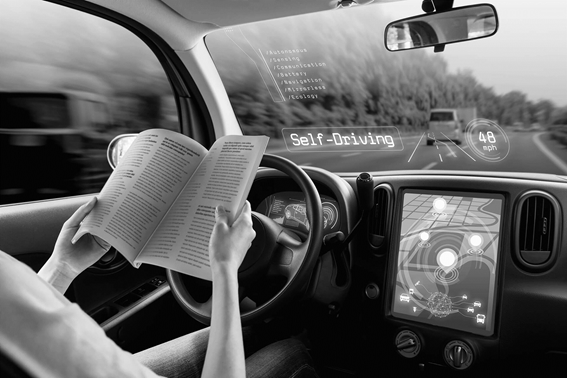
\includegraphics{future3.png}
\caption{Sistema de transportes inteligentes.}
\label{fig_futuro3}
\end{figure}


-----------------------------------------------------------------------------------------------\\


\chapter{Estado da Arte}


\section{Introdução}
%%%%%%%%%%%%%%%%%%%%%%%%%%%%%%%%%%%%%%%%%%%%%%%%%%%%%%%%%%%%%%%%%%%%%%%%%%%%%%%%%%%%%%%%%%%%%%%%%%%


%%%%%%%%%%%%%%%%%%%%%%%%%%%%%%%%%%%%%%%%%%%%%%%%%%%%%%%%%%%%%%%%%%%%%%%%%%%%%%%%%%%%%%%%%%%%%%%%%%%

\chapter{Condução autónoma no Festival Nacional de Robótica}

\section{Introdução}

O Festival Nacional de Robótica é uma iniciativa da Sociedade Portuguesa de Robótica, teve a sua primeira edição em 2001 e que tem como objetivo divulgar a Ciência e a Tecnologia junto dos jovens dos ensinos básico, secundário e superior, bem como do público em geral, por intermédio de competições de robôs e contribuir para o desenvolvimento da investigação nas áreas da Robótica e da Automação. Este Festival realiza-se todos os anos numa cidade diferente, tendo desde a sua primeira edição passado pelas cidades de Guimarães, Aveiro, Lisboa, Porto, Coimbra entre outras. 

As provas que decorrem ao longo do festival envolvem o domínio de componentes técnicas com graus de dificuldade distintos, razão pela qual as várias provas foram distribuídas em dois tipos de competições: sénior e júnior.

As provas da competição júnior são as provas de busca e salvamento, dança e futebol robótico. Por seu lado, as provas que compõem a competição sénior são as provas de condução autónoma, da liga de robôs médios de futebol robótico.

A prova de Condução Autónoma

A prova de Condução Autónoma desenrola-se em três fases, sendo em cada uma delas, necessário completar duas voltas a uma pista que pretende simular, tanto quanto possível, uma estrada convencional. 

\begin{figure}[H]
\centering
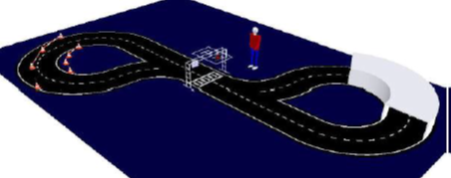
\includegraphics{pista_FNR.png}
\caption{O Demonstrador para carros autonomos.}
\label{fig1_FNR}
\end{figure}

A pista tem a forma aproximada de um oito, é delimitada tanto interior como exteriormente por linhas contínuas brancas, tem duas faixas de rodagem separadas por um traço interrompido, uma passadeira e um par de painéis sinaléticos (um em cada sentido), que funcionam como semáforos. 

\begin{figure}[H]
\centering
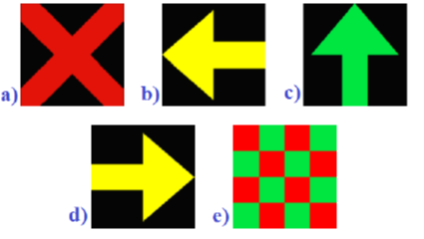
\includegraphics{signals_FNR.png}
\caption{O Demonstrador para carros autonomos.}
\label{fig2_FNR}
\end{figure}

De fase para fase da competição são introduzidos novos desafios com os quais os robôs têm de lidar (obstáculos sobre a faixa de rodagem, um túnel sobre uma das curvas, uma zona de obras e uma área de estacionamento).

\begin{figure}[H]
\centering
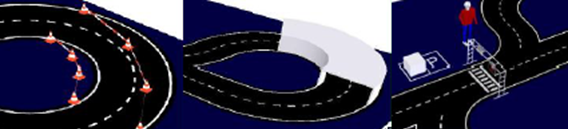
\includegraphics{Desafios_FNR.png}
\caption{Desafios propostos FNR.}
\label{fig3_FNR}
\end{figure}

Condução autónoma no FNR (Festival Nacional de Robótica)

A condução autónoma especificada baseia-se nos seguintes parâmetros. A pista é definida por uma faixa de rodagem delimitada por duas linhas contínuas. Esta mesma faixa é dividida por uma linha tracejada (ou por vezes continua) equidistante das duas faixas delimitadoras e que define dois sentidos de condução. No centro da pista encontra-se a representação de uma passadeira sobre a qual estão expostos dois monitores (um para cada sentido) que podem apresentar variadas sinalizações predefinidas. Junto a esta localização, logo após a passadeira, e apenas num dos sentidos está definida uma zona de parqueamento do robô fora da faixa de rodagem. Estes detalhes (que podem ser identificados na Figura XX - 

\begin{figure}[H]
\centering
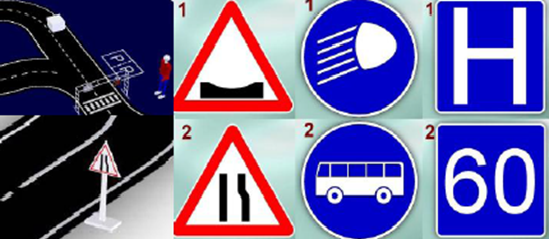
\includegraphics{sinais_transito_FNR.png}
\caption{Sinais de Transito utilizados no demonstrador do FNR.}
\label{fig4_FNR}
\end{figure}

Exemplo de pista para condução autónoma.) são gerais e não são alterados ao longo de toda a competição.  



-----------------------------------------------------------------------------------------------\\
-----------------------------------------------------------------------------------------------\\

\codeFile{treta}
\pyFile{treta}
%\printbibliography
%\bibliographystyle{plainnat}
\bibliography{XBib}
\end{document}
%-----------------------------------------------------------------------
